\begin{myex}
		La fonction $f(x) = \dfrac{1}{2}x + 3$ est croissante sur $\intervOO{- \infty }{+ \infty}$.
		\begin{center}
			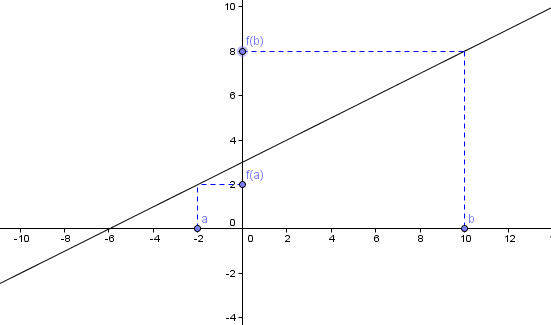
\includegraphics[scale=0.65]{./img/croiss}
		\end{center}
		
		\begin{itemize}
			\item $a$ et $b$ appartiennent à $\intervOO{- \infty }{+ \infty}$, on a $a \leq b$ donc $f(a) \leq f(b)$.
			\item $-2 \leq 10$ donc $f(-2) \leq f(10)$ ($2 \leq 8$).
		\end{itemize}
		
\end{myex}